%\vspace{1.5\baselineskip}
\begin{figure}[H]
    \begin{center}
    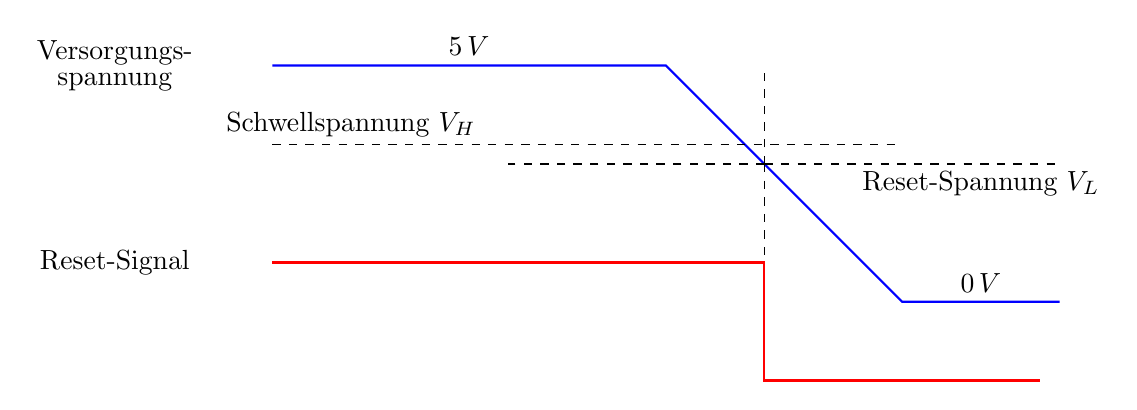
\begin{tikzpicture}
        % Achsen
        % \draw[->] (0,0) -- (10,0) node[anchor=north] {s}; % x-Achse
        % \draw[->] (0,0) -- (0,4) node[anchor=east] {V}; % y-Achse

        % Linie
        \draw[thick, blue] 
            (0,3) -- (5,3) % waagerechter Teil von 0 bis 2 Sekunden
            to (8,0) -- ++(2,0);
            % Kreuzungspunkt berechnen
        \coordinate (Kreuzung) at (6.25,1.75);

        
        \draw[thick, red] 
            (0,0.5) -- ++(6.25,0) -- ++(0,-1.5) -- ++(3.5,0);

        % Gestrichelte Linien
        \draw[dashed] 
            (Kreuzung) -- ++ (-3.25,0)
            (Kreuzung) -- ++ (3.75,0); % Waagerechte Linien
        \draw[dashed] 
            (Kreuzung) -- ++(0,-1.25)
            (Kreuzung) -- ++(0,1.25); % Senkrechte Linien
        \draw[dashed] (0,2) -- ++ (8,0); % Schwellspannung
            
        % Beschriftungen
        \node[anchor=south, xshift=-1cm] at (10,0) {$0\,V$}; % Startpunktbeschriftung
        \node[anchor=south] at (2.5,3) {$5\,V$}; % Endpunktbeschriftung
        \node[] at (-2,3) {\shortstack{Versorgungs- \\spannung}};
        \node[] at (-2,0.5) {\shortstack{Reset-Signal}};
        \node[] at (1,2.25) {\shortstack{Schwellspannung $V_H$}};
        \node[] at (9,1.5) {\shortstack{Reset-Spannung $V_L$}};
        
    \end{tikzpicture}        

    \end{center}
    \caption[Reset-Spannung]{\\Quelle: Reset-Spannung (Eigene Darstellung)}
    \label{fig:Reset-Spannung}
\end{figure}
%\vspace{1.5\baselineskip}